% Copyright (C)  2016 Philipp Hacker.
% Permission is granted to copy, distribute and/or modify this document
% under the terms of the GNU Free Documentation License, Version 1.3
% or any later version published by the Free Software Foundation;
% with no Invariant Sections, no Front-Cover Texts, and no Back-Cover Texts.
% The lincense itself can be found at <https://www.gnu.org/licenses/fdl-1.3>.

\documentclass[a4paper,10pt]{article}
%\documentclass[numbers=noenddot,12pt,a4paper,notitlepage,twoside,BCOR15mm]{scrartcl}

\usepackage{lipsum}
\usepackage{multicol}

\usepackage[T1]{fontenc}
\usepackage[utf8]{inputenc}

\usepackage[infoshow]{tabularx}
\usepackage[all]{xy}

\usepackage{geometry}
\geometry{%
	a4paper,
	left=24mm,
	right=24mm,
	top=24mm,
	bottom=24mm,
	}

\usepackage{amsmath,mathtools}
\usepackage{amssymb}
\usepackage{units}
\usepackage{upgreek}
\usepackage{esint}
\usepackage{graphicx}
\usepackage{ziffer}

\usepackage{float}
\usepackage{lscape}

\usepackage[labelfont=bf]{caption}
\usepackage{wrapfig}
\usepackage{subcaption}

\usepackage[backref=page]{hyperref}

\usepackage{csquotes}
\usepackage[infoshow]{tabularx}
\usepackage{fancyhdr}

\usepackage{sectsty}
\usepackage{times}

\usepackage{lmodern} %TODO Schriftart
\usepackage[greek,english]{babel} %TODO Sprache einstellen

\renewcommand{\headrulewidth}{0.1pt}
\renewcommand{\footrulewidth}{0.1pt}
\newcommand{\name}{\text{Philipp Hacker}} %TODO Name des Protokollanten eintragen

\setlength{\parindent}{0pt}

\newcommand{\degree}{^\circ}
\newcommand{\diff}{\textnormal{d}}
\newcommand{\tenpo}[1]{ 10^{#1}}
\newcommand{\greek}[1]{\greektext#1\latintext}
\newcommand{\ix}[1]{_\text{#1}}
\newcommand{\imag}{\mathbf{i}}
\newcommand{\tilt}[1]{\textit{#1}}
\newcommand{\grad}[1]{\textit{grad}\left(#1\right)}
\newcommand{\divergenz}[1]{\textit{div}\left(#1\right)}
\newcommand{\euler}{\mathnormal{e}}
\newcommand{\fett}[1]{\textbf{#1}}
\newcommand{\ket}[1]{|#1\rangle}
\newcommand{\bra}[1]{\langle#1|}

\newcommand{\HRule}{\rule{\linewidth}{0.5mm}} % New command to make the lines in the title page

\author{Philipp Hacker} % Your name, this is used in the title page and abstract, print it elsewhere with \author

\newcommand{\prof}{Prof. Dr. Meichsner}

\newcommand{\supname}{Dr. S. Nemschokmichal, R. Tschiersch} % Your supervisor's name, this is used in the title page, print it elsewhere with \supname

\newcommand{\univname}{Ernst-Moritz-Arndt University Greifswald} % Your university's name and URL, this is used in the title page and abstract, print it elsewhere with \univname

\newcommand{\deptname}{Institute of Physics} % Your department's name and URL, this is used in the title page and abstract, print it elsewhere with \deptname

\newcommand{\groupname}{Low-temperature Plasma Physics group} % Your research group's name and URL, this is used in the title page, print it elsewhere with \groupname

\newcommand{\rtitle}{Electric field strength spectroscopy in dielectric barrier discharges}

\date{\today}


\pagestyle{fancy}
\fancyhead[R,L,C]{}
\fancyfoot[R,L,C]{}
\fancyhead[RE]{\href{http://www.physik.uni-greifswald.de/}{\deptname}}
\fancyhead[LO]{\href{http://www1.physik.uni-greifswald.de/}{\groupname}}
\fancyhead[LE]{\today}
\fancyfoot[LO, RE]{\thepage}
\fancyfoot[LE, RO]{Section \thesection}

\begin{document}

	\setcounter{section}{-1}
	
	\renewcommand*{\contentsname}{Table of Contents}
	\renewcommand*{\equationautorefname}{eq.}
	\renewcommand*{\figureautorefname}{fig.}
	\renewcommand*{\tableautorefname}{tab.}
	\renewcommand*{\sectionautorefname}{sec.}
	\renewcommand*{\subsectionautorefname}{subsec.}
	\renewcommand*{\subsubsectionautorefname}{subsec.}
	\renewcommand*{\figurename}{Fig. }
	\renewcommand*{\tablename}{Tab. }

	\renewcommand*{\figurename}{Figure }
	\renewcommand*{\tablename}{Tabel }

	
	\thispagestyle{empty}
	
	\begin{center}
			
			\HRule \\[0.4cm] % Horizontal line
			\huge \fett{\rtitle} \\ % Thesis title
			\HRule \\[.6cm] % Horizontal line
			
			\large \href{http://www.university-url.com}{\univname}

	\begin{figure}[h]
		\centering
		
		\begin{minipage}[t]{0.48\textwidth}
			\begin{center}
			\emph{Author}: \href{https://github.com/RayleighsJeans/ag_praktikum_2016}{\name} \\ %TODO author
			\emph{Examiner:} \prof
			\end{center}
		\end{minipage}
		\hfill
		\begin{minipage}[t]{0.48\textwidth}
			\begin{center}
				\emph{Supervisor}: Dr. S. Nemschokmichal,\\R. Tschiersch \\ %TODO name of supervisor
			\end{center}
		\end{minipage}
	\end{figure}

		\large \textit{Report for an internship at the \groupname \,\, of Prof. Dr. Meichsner, submitted in fulfillment of the requirements for the degree}\\[0.1cm] \fett{Master of Science}\\[0.2cm] %TODO UNIVERSITY TEXT
		\textit{in the}\\[0.2cm]
		\href{http://www1.physik.uni-greifswald.de}{\groupname} \\[0.15cm] \href{http://www.physik.uni-greifswald.de}{\deptname} \\[0.3cm] %TODO RESEARCH GROUP/DEPARTMENT

	\end{center}
	
		\vspace{1cm}
	
	\begin{multicols}{2}
		\tableofcontents
	\end{multicols}
	
		\vspace{1cm}
	
		\section{Abstract}
		
	\twocolumn

	\section{Introduction}

		In the vast field of low temperature plasma physics, barrier discharges (\tilt{BD}s) take a special place as a result to their unique feature of surface charge deposition onto, in dielectric covered electrodes. During the discharge breakdown, the accumulated charges limit the overall current, as they weaken the, in opposite direction applied electric field. Furthermore, by that means these plasmas are thermally non-equilibrated, even at atmospheric pressures. Hence, they are source of many different radicals, excited species and high energy electrons and photons. In addition, a variety of working gases and their combinations can be used to dominantly determine the discharge modes, each yielding characteristic physical quantities, obtainable through, e.g. non-invasive optical spectroscopy or external measurements of electrical properties.\\ 
		Barrier discharges are very attractive to the industry due to their comparatively low power consumption, almost at normal residing electron temperatures and easy-to-achieve viability. They are a lucrative mean to a broad selection of industrial, high quality productions, in e.g. for surface treatments, gas synthesis, or in life science.\\
		Specifically speaking, certain properties of \tilt{BD}s, like short, non-stationary breakdown times and therefore fast repeatability, statistical behavior and non-thermal distribution functions, motivate the intense study of the many phenomena found in dielectric hindered, atmospheric-pressure, low temperature\linebreak plasmas.\\
		By variation of the discharge configurations, such as electrode spacing, applied voltage, gas flow and mixture or dielectrics, a \tilt{BD} can be operated with filamentary micro discharges (\tilt{MD}s), which appear as thin, lateral expanded filaments, or in diffuse modes. The latter will be subject of my investigation. Here, one finds the atmospheric pressure Townsend-like discharge (\tilt{APTD}) and the atmospheric pressure glow-like discharge (\tilt{APGD}).\\
		\tilt{APTD}s are mostly investigated in rare gases with high ionization inside the discharge volume at a low electric field strength. Essentially, elementary multistage processes of such noble gases account for many metastable species, which are found to be crucial to the \tilt{BD}s characterization. A unique feature is the development of a cathode fall region during the breakdown.\\
		\tilt{APTD}s are result to a high ratio of secondary electron emission to volume ionization. This is caused by the Townsend breakdown at the cathode, primarily in gases with metastable species which have enough energy to produce secondary electrons, yielding a exponential growth of electron density towards the anode.\\
		The Townsend-like and the glow-like discharge separate each other by a difference in transferred current during the breakdown of at least one magnitude. Therefore, the knowledge of such plasma properties and their dependence on discharge conditions is a important point for applications, as already sketched. In addition to the measurement of external quantities, electron temperatures, plasma currents and densities or produced species, the spatially resolved investigation of the resulting electric field strength, and therefore related characteristics like optical emission and life time, becomes cruel to the true understanding of the discharge. Concretely, any macroscopic electric fields in plasmas are result of space charge formation. Their characteristics commonly determine the energy flux of charged particles and therefore, the behavior of the discharge itself. \\
		On the one hand, electric field strength measurements through experimentally determined distributions of emission intensities have been appointed as standard, though this method is limited to a small region of nitrogen to oxygen ratios, only applicable in \tilt{MD}s. On the other hand, for a long time, experimental fusion devices relate on the helium line intensity ratio method to determine electron densities, temperatures and the local electric field strength. In fact, electron impact excitations are insensitive to electron density but to electron temperature. If one uses the ratio of two line intensities excited in the plasma, the electron density factor gets cancelled out and what remains is only dependent on the electric field strength. Hence, this method can be used to obtain a field strength distribution in spatially small dielectric barrier discharges at low temperatures and atmospheric pressures.\\
		In this case, Helium is used, as the singlet spin state weakly depends on an initial metastable population. To irrefutably receive a proper field strength from this measurement, a collisional-radiative model has to be utilized to obtain and confirm any functional dependence of the surveyed quantities.\\
		Furthermore, a second method for electric field \linebreak strength measurement will be introduced. Stark splitting and shifting of atomic levels, therefore their spectroscopic emission lines, is a well established method in plasma diagnostics. It is based solely, so to speak \tilt{ab initio} on nature, on the quantum mechanical perturbation of atomic energy levels by strong external electric fields. Hence, neither equilibrium or additional conditions have to be fulfilled, nor is the line splitting a function of other plasma properties other than field strength. Polarization filters are used to distinguish between the different $\pi$ and $\sigma$ bands, as a full spectrum may include overlaps, which can lead to misinterpretation.\\
		Here, the linear Stark effect can be applied on the splitting of $\pi$-polarized, forbidden and allowed energy levels in Helium atoms. A polynomial will be used to fit the splitting to the field strength. The allowed-forbidden gap will be investigated at around $\unit[492,2]{nm}$ for the transition 1s2p$^1$P$^0$ - 4d$^1$D$^0$ and its forbidden counterparts 2p$^1$P$^0$ - 4p$^1$P$^0$ and 2p$^1$P$^0$ - 4f$^1$F$^0$.\\
		In this report, a comparison of spatially and temporally high resolved measurements, in both the two ways mentioned above, will be done. This is part of the \tilt{internship} at the \groupname\,\,of Prof. Dr. Meichsner. It is crucial to find a qualitative agreement in the results, as this would satisfy each methods theories, as well as the diagnostics set up. Overall, the main goal should be to experience and exercise correct and conscientious scientific research on a regular basis.\\
		The outline of this report is as followed. In the next section, the experimental set-up that was used and the diagnostics will be briefly reviewed. Section 3 consists of the presentation of selected results, associated discussion of such, as well as the final conclusion to this internship.

	\section{Experimental set up}
	
		\subsection{Discharge configuration}
		
				\begin{figure}[t]
					\centering
					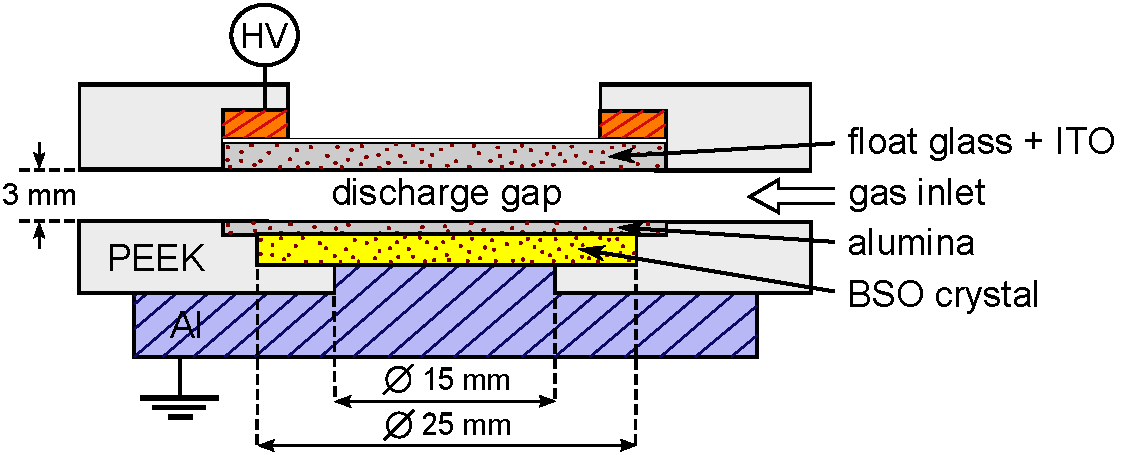
\includegraphics[width=0.5\textwidth]{figures/experimentalsetup/discharge_cell.pdf}
					\caption{side-view of the concentric discharge cell. The variable dielectric was chosen to be mono-crystalline alumina.}
					\label{img:cell}
				\end{figure}
		
			The used discharge cell is shown in \autoref{img:cell}. An symmetrical configuration, in which both plane, concentric electrodes are covered in dielectrics. The gas gap is $\unit[3]{mm}$ in height, whereas the radius of the electrodes is $\unit[15]{mm}$. A high-voltage driven copper ring on top holds a float glas plate, which is again covered with a electrically conductive, transparent indium tin oxide  (\tilt{ITO}) layer. On the bottom, a grounded aluminium mirror holds a bismuth silicon oxide crystal (\tilt{BSO}). On top of that, the dielectric can be mounted. Here, \tilt{mono-crystalline alumina} (Al$_2$O$_3$) was used. In advance for further investigations, one finds the relative permeabilities of the materials to be $\epsilon_r=7,6$ for the float glas + ITO and $\epsilon_r=10,55$ for the aluminum.\\
			The whole construct is mounted inside a steel vacuum chamber. A turbomolecular and process pump evacuate the chamber to a base pressure of about $\unit[\tenpo{-5}]{mbar}$, which ensures low concentration of impurities. Afterwards, the operating gas is passed from one side directly into the chamber through the polyetherethereton (\tilt{PEEK}) insulaters. Two mass flow controllers (MKS 647c) set the gas flow rate of Helium and Nitrogen (respective purity > 99,999\%) achieving high accuracy mixtures and flow rates of up to $\unit[100]{sccm}$. The operating pressure was at atmospheric level, $\unit[1000]{mbar}$ and kept constant through a diaphragm pressure gauge and butterfly valve (MKS) by the process pump (TRIVAC D25BCSPFPE). Moreover, 2 orifices in the chamber enable the gas flow and investigation of the discharge.\\
			A function generator (SRS DS345) provides the voltage signal for the upper electrode, which ignites the discharge after its been amplified by a factor of 1000 (Trek 615-10), at a frequency of $\unit[5]{kHz}$ and amplitude of $\unit[1,2]{kV}$. The voltage can be a sine or square wave, dominating the discharge modes.\\
			Applied voltage $U_{app}(t)$ and total transported charge $Q_{ext}$ are measured via a HV probe of 1000:1 and an external capacitor as well as a resistor, $C_{ext}=\unit[1]{nF}$ and $R_{ext}=\unit[100]{\Omega}$. The collection of data itself is utilized by a digital oscilloscope (ROHDE\&SCHWARZ RTO1024) with a bandwidth of $\unit[2]{GHz}$, which is connected through ethernet ports to a PC, running a customized LabView VI. Additionally, a Rogowski coil is attached to the cell, accumulating the flowing current and providing a much faster and higher slope in voltage signal than the total charge or the ramping of the applied voltage. This will also be used as the trigger for the oscilloscope.
			
				\begin{figure}[t]
					\centering
					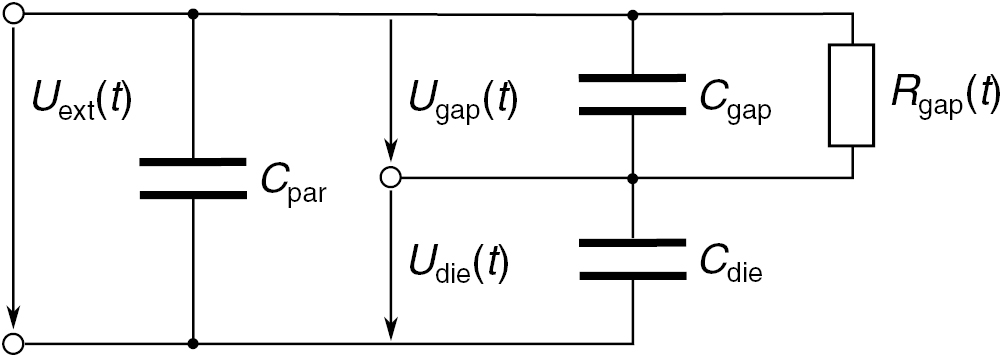
\includegraphics[width=0.5\textwidth]{figures/experimentalsetup/replacementcircuit.jpg}
					\caption{Electrical equivalent circuit: the discharge gap is represented by the time-dependent resistance $R_{gap}(t)$ and $C_{gap}$ in parallel.}
					\label{img:circuit}
				\end{figure}
			
			 Furthermore, by using Lissajous figures $Q(U)$, one gains access to the breakdown charge $\Delta Q$ and the determination of the total capacitance of the discharge cell $C_{tot}$. By that, the gap voltage between the dielectrics $U_{gap}$ and the displacement current $I_{dis}$ can be calculated. A replacement circuit can be constructed, as depicted in \autoref{img:circuit}. Here, $C_{diel}$ and $C_{gap}$ denote the dielectrics and discharge gap capacitance, taking into account the geometry. The parallel capacitance $C_{par}=C_{tot}-C_{gap}C_{diel}/\left(C_{gap}-C_{diel}\right)$ comprehends any volume in the cell not ignited by the discharge. Finally, one yields:
			 
			 	\begin{align}
					&U_{gap}(t)=\left(1+\frac{C_{par}}{C_{diel}}\right)U_{ext}(t)-\frac{Q_{ext}(t)}{C_{diel}} \nonumber \,\, , \\
					&I_{dis}(t)=\left(1+\frac{C_{gap}}{C_{diel}}\right)\left(\frac{\diff Q_{ext}(t)}{\diff t}-C_{tot}\frac{\diff U_{ext}(t)}{\diff t}\right) \nonumber \,\, .
				\end{align}

		\subsection{Optical emission spectroscopy}
		
				\begin{figure}
					\centering
					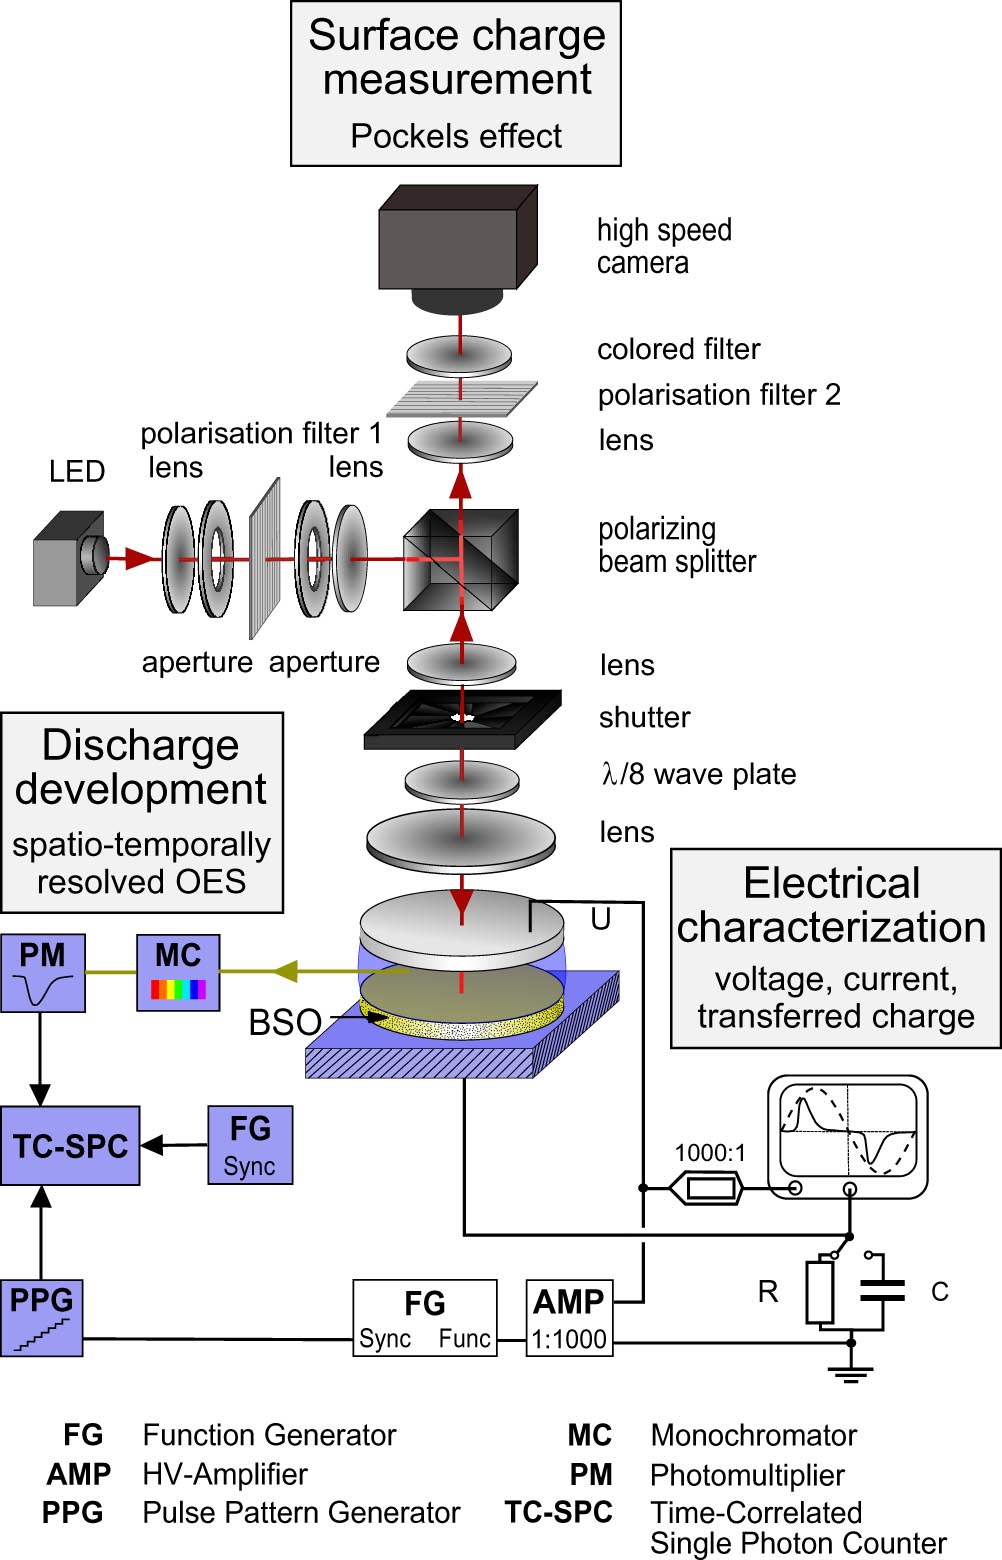
\includegraphics[width=0.5\textwidth]{figures/experimentalsetup/diagnostic_setup.jpg}
					\caption{Set-up of the diagnostics applied at the discharge cell configuration.}
					\label{img:diag}
				\end{figure}
		
			The \autoref{img:diag} illustrates the diagnostic set-up, by which the simultaneous investigation of electrical quantities, like charge and current, as well as the optical emission from the discharge is possible.\\			Here, spatio-temporally resolved single photon counting becomes accessible through a high-gain photomultiplier (\tilt{PM}: Becker\&Hickl PMH-100), a 1:1250 amplifier and monochromator. The fully movable optical system of two lenses, one slit and three nonius screws for vertical and horizontal adjustments across the full discharge cell, is focused via 1:-1 onto the monochromator (\tilt{MC}: Horiba, Triax 320). In this case, a spatial resolution of $\unit[0,1]{inch}$ and $\unit[0,15]{inch}$ is chosen. Through the combination of rogowski coil and digital oscilloscope a temporal resolution down to $\unit[2]{ns}$ is achieved. With a gratin of $\unit[2400]{mm^{-1}}$, the monochromator achieves a spectral resolution of $\unit[0,02]{nm}$ at comparable low intensities. At $\unit[1800]{mm^{-1}}$ one yields a lower resolution with higher intensities.\\
			As the discharge frequency was chosen to be $\unit[5]{kHz}$, many data acquisitions per second can be performed by the digital oscilloscope. As the PM achieves a individually distinguishable electric signal for each photon, the raw data from the PM and amplifier has to be averaged over thousands of inner loops - for example 28000 averages at a sample rate of $\unit[100]{MSa/s}$. This cancels out a lot of the statistic noise, caused by any unwanted light through the chambers cover. In addition, outer loops will be done to rule out medium-range perturbations.\\
			For the line emission intensity ratio spectroscopy, the monochromator first scans a full spectrum between $\unit[585-730]{nm}$, including all Helium lines of interest. Specifically, those will be: He I $\unit[587,65]{nm}$ ($2^3$P$-3^3$D) and He I $\unit[706,66]{nm}$ ($2^3$P$-3^3$S) triplet, as well as He I $\unit[728,31]{nm}$ ($2^1$P-$3^3$S) and He I $\unit[667.98]{nm}$ ($2^3$P$-3^3$S) singlet. Surprisingly, those lines come with a small offset of $\approx\unit[0,15]{nm}$, compared to values obtained from various literature. This will be further discussed in the next section.\\
			While the line ratio measurement is based of a single wavelength, the Stark spectroscopy passes a small window of $\unit[0,7]{nm}$ in $\unit[0,02]{nm}$ steps. Therefore, the spectral resolution is much higher, whereas the intensity becomes smaller by many magnitudes.\\
			Both methods use the same set up, but differ in application. During the line emission spectroscopy, the optical system is elevated each time the measurement of all four lines is completed. Therefore, the entrance and exit slit of the MC are widened to $\unit[0,2]{mm}$ and vertically opened to $\unit[1]{mm}$. This way the cell gap is scanned with $\unit[0,05]{inch}$ steps.\\
			For Stark spectroscopy, the entrance/exit slit height is maxed to $\unit[3]{mm}$, resulting in a lower spatial resolution of $\unit[0,1]{inch}$. Furthermore, the already mentioned polarization filter is placed along the optical axis between the MC and discharge cell.

	\section{Results}

		\subsection{Overview spectrum of optical emission}
		
		\begin{itemize}
			\item Benennen der einzelnen Peaks mit 'Übergang' + Wellenlänge (volle Seitenbreite); YAchse --> intensity, a.u. + Normierung auf Maximum
			\item aus Literatur: weitere Übergänge identifizieren
			\item TEXT: Arbeitsbedingungen (Entladung, Gase, Flussraten, Signalform, Amplitude etc...); wie das 'integrierte' Spektrum erstellt wurde; dominante Linien im Spektrum --> Helium (Elektronen-Stoß-Ionisation) + Art und Verlauf der Abregung; weitere Übergänge (andere System von N2/He2/O2/H2O ...) beschreiben + Grund (ohne explizite Formulierung der RG
		\end{itemize}
		
		\subsection{Spatio-temporally resolved optical emission}
		
		\begin{itemize}
			\item Zeitskala bei 2016-06-20 bearbeiten (-6$\mu$ s-14$\mu$s); vertikale Positionen mit Kathode/Anode kennzeichnen (oben:K, unten:A)
			\item was ist dargestellt (Konfiguration, Arbeitsbedingungen...)?
			\item Gemeinsamkeiten \& Unterschiede für Strom-Spannungs-Kennlinien: Anstiege der angelegten Spannungen, aber gleiche Spannungsamplitude; berechnete Durchbruchspannung aus $U_{gap}$ unterschiedlich; Einbruch der Gap-Spannung während des Durchbruchs, jedoch unterschiedlich stark <--> Abfluss der erzeugten Volumenladungen und Deponierung auf den Dielektrika --> Gegenfeld; starker Einbruch der Spaltspannung --> glimmartige Entladung <--> hohe Ionisation im Volumen (Gegensatz zu Townsend: konstante Spaltspannung während des Durchbruchs, da Sekundärelektronenemissionen signifikant: GG aus Strom von Oberfläche und Entladung); hohe Flüsse von Ladungsträgern auf die Elektroden; höherer Abfall in Spaltspannung bedeutet intensivere Entladung auf Grund von mehr erzeugten deponierten Ladungen; wesentlich niedrigerer Stromamplitude bei Sinusentladung aber längere Strompulsdauer (wg. niedrigerer Durchbruchspannungen); längere Anstiegszeit in der angelegten Spannung --> Strompulsdauer; längere Vorphase in der Sinusentladung --> mehr Akkumulation von Ladungen im Volumen, deswegen insgesamt niedrigere Durchbruchspannung; 
			\item Gemeinsamkeiten \& Unterschiede für Raum-Zeit aufgelöste Emissionen:
					ZEITLICH GEORDNET:	- während der Vorphase schwaches Emissionmaximum vor der Anode (Tonwsend-Vorphase, exponentielle Elektronenvervielfältigung in Richtung Anode, nahezu homogenes Feld über dem Gasspalt)
															- Entwicklung positiver Raumladung vor der Anode (träge Ionen gegen mobile Elektronen) --> kathodengerichtete Ionisationsfront (Durchbruch) 
															- während des Strommaximums, folgt: Emissionsmaxima vor der Kathode während des Durchbruchs (negative glow); dazu Leuchterscheinung zur Anode hin --> positive Säule (kurzzeitger Stromfluss über das Volumen, bei Rechteckspannung); niedrige Feldstärke, da Quasineutralität nahezu erfüllt in pos. Säule;  bei Sinus: keine positive Säule; Ionisationsfront bei Rechteck schnell genug, womit Ladungsträger im Spalt ausreichend (im Volumen), um viel Strom zu transportieren 
															- Nachphase (after glow) vor der Kathode weitaus länger;  
		\end{itemize}
		
		\subsection{Line ratios}
		
		\subsection{Stark spectroscopy}

		\subsection{Conclusion}
		
	\section{References}

		\bibliography{report.bib}
		\bibliographystyle{unsrt}

	\section{Appendix}


\end{document}